\documentclass[a4paper,12pt]{article}

\usepackage[russian]{babel}
\usepackage{cmap}
\usepackage[utf8]{inputenc}
\usepackage[usenames]{color}
\usepackage{tabularray}
\usepackage{xcolor}
\usepackage{graphicx} 
\usepackage{subfigure}
\usepackage{subcaption}

\usepackage[unicode]{hyperref} % цвета гиперссылок
\hypersetup{
	colorlinks,
	citecolor=black,
	filecolor=black,
	linkcolor=blue,
	urlcolor=black
}

\usepackage{geometry} % задаёт поля 
%\geometry{left=3cm}
%\geometry{right= 1.5cm}
%\geometry{top=2cm}
%\geometry{bottom=2cm} 

\usepackage{enumitem} % настраивает работу со списками:
\def\labelitemi{—} % ... задаёт длинное тире как стандартный маркер ненумерованного списка
\setlist{nolistsep} %  ... убирает дополнительный отступы между элементами списка


% удаляет названия и продолжение следует и т. для таблиц, будет только таблица без всего
\DefTblrTemplate{contfoot-text}{default}{}
\DefTblrTemplate{conthead-text}{default}{}
\DefTblrTemplate{caption}{default}{}
\DefTblrTemplate{conthead}{default}{}
\DefTblrTemplate{capcont}{default}{}


\title{Разбиение данных о потреблении контента на оптимальное число кластеров}
\author{В. Г. Мосин}
\date{}

%   \input{preamble.tex}
\begin{document}
	\maketitle
	\abstract{\noindent  Исследован метод определения оптимального числа кластеров при выполнении кластеризации KMeans. Предложена метрика эффективности разбиения, изложены последовательные шаги алгоритма для ее вычисления. На примере данных о потреблении контента пользователями одного из ведущих хостингов показана состоятельность предложенного метода. }
	
\tableofcontents
	
\section{Введение}
Определение количества кластеров в алгоритмах кластеризации — это важный этап анализа данных, который требует обдумывания и экспертных оценок. Часто определение количества кластеров происходит на основе интуиции или предварительных знаний о данных и задаче. У ученых и экспертов в области данных может быть опыт или понимание, которое помогает им сделать предположение о подходящем количестве кластеров (см. [3]).

Однако часто бывает необходимо исключить экспертную оценку (например, если кластеризация осуществляется в рамках более сложного алгоритма в режиме реального времени) и настроить гиперпараметры алгоритма кластеризации, основываясь на объективных методах, а не на человеческой интуиции.

Один из подходов к решению этой задачи рассматривается в настоящей статье.


\subsection{Теоретическая часть}

Несмотря на то, что кластеризация данных относится к задачам машинного обучения без учителя, и, тем самым, не требует разбиения данных на обучающую (то есть, заранее размеченную) и тестовую выборки, мы произведем такое разбиение для того, чтобы получить возможность сравнить два результата кластеризации. Если результаты окажутся близкими, мы будем считать, что разбиение проведено на верное число кластеров, в противном случае будем пытаться подобрать другое разбиение (см. [2]).

Для сравнения различных разбиений нам понадобится некоторая метрика их качества, и чтобы ее получить, мы вводим две матрицы принадлежности, которые показывают, принадлежат ли два объекта одному кластеру, или же они принадлежат разным кластерам.


\subsubsection{Матрица принадлежности \texttt{M\_train\_test}} 

Итак, мы разбили данные на обучающую и тестовую выборки. Обучаем алгоритм KMeans на обучающей выборке и применяем обученный алгоритм к тестовой выборке. После этого каждый объект тестовой выборки получает метку принадлежности к тому или иному кластеру. Матрица \texttt{M\_tyrain\_test} определяется как квадратная матрица, порядок которой равен объему тестовой выборки, а элемент с номером $(i, j)$ равен 1, если метки $i$-го и $j$-го объектов равны между собой, или 0, если они различны.


\subsubsection{Матрица принадлежности \texttt{M\_test}} 

Обучаем алгоритм \texttt{KMeans} на тестовой выборке и применяем обученный алгоритм к ней самой. После этого каждый объект тестовой выборки получает метку принадлежности к тому или иному кластеру. Аналогично предыдущему пункту матрица \texttt{M\_test} определяется как квадратная матрица, порядок которой равен объему тестовой выборки, а элемент с номером $(i, j)$ равен 1, если метки $i$-го и $j$-го объектов равны между собой, или 0, если они различны.

Теперь у нас есть две матрицы принадлежности одного для одного и того же набора объектов. Разумно предположить, что разбиение проведено качественно, если эти матрицы похожи друг на друга. И наоборот: если они сильно отличаются, разумно предположить, что такое разбиение менее качественно.

\subsubsection{Метрика качества разбиения} 

Рассмотрим разность матриц:

\medskip\noindent
\texttt{M\_train\_test – M\_test}

\medskip\noindent
Понятно, что чем больше в ней нулей, тем более они похожи. Вычисляем количество нулевых элементов в разности матриц принадлежности и, чтобы получить возможность сравнивать результаты кластеризации на множествах разных объемов, нормализуем это число путем деления на общее количество компонент (то есть, на квадрат объема тестовой выборки). То, что получается в результате — это доля совпадений в матрицах принадлежности. Именно ее мы будем использовать как оценку качества разбиения: чем ближе доля совпадений к единице, тем качественнее разбиение.

\subsection{Постановки задачи}

\subsubsection{Предмет исследования}Исследуется прогнозирующая способность нескольких регрессионных моделей до и после удаления выбросов. 

\subsubsection{Методика исследования} Мы будем последовательно вычислять метрику качества в разных ситуациях и сравнивать получающиеся результаты. Поскольку, результаты естественным образом зависят от двух параметров:

\medskip\noindent 

\begin{enumerate}
	\item от числа кластеров, на которые проводится разбиение,
	\item от пропорции, в которой разбиваются данные на обучающую и тестовую выборки,
\end{enumerate}

\medskip\noindent 
наша методика будет состоять в выполнении вложенного цикла: внутренний цикл мы будем вести по объему тестовой выборки, а внешний — по числу кластеров.

\subsubsection{Цель исследования} 

Наша цель — продемонстрировать эффективность предложенного метода на примере данных о потреблении контента пользователями одного из ведущих хостингов.

\subsection{Библиотеки}
Для выполнения вычислений и анализа данных мы пользуемся средой \texttt{Jupyter Notebook}, которая предоставляет удобные средства для работы с языком программирования Python и его главными библиотеками: \texttt{NumPy}, \texttt{Pandas}, \texttt{sklearn} и \texttt{matplotlib}. Благодаря этим инструментам, мы можем эффективно работать с данными, выполнять исследования и визуализировать результаты (см. [1], [2]). 

%Библиотека \texttt{numpy} является одной из ключевых библиотек для научных вычислений и обработки массивов данных в языке программирования \texttt{Python}. Библиотека \texttt{pandas}~--- одна из наиболее популярных и мощных библиотек для работы с данными в языке программирования \texttt{Python} (см. [1]). 

%Библиотека \texttt{scikit-learn}, широко известная как \texttt{sklearn}, предоставляет обширный набор инструментов и функций для решения различных задач в языке программирования Python, таких как задачи классификации, регрессии, кластеризации и др. Мы используем эту библиотеку для решения регрессионных задач.

\section{Описание данных}
В качестве данных для исследования используются сведения о потреблении контента пользователями одного из ведущих хостингов. Данные содержат записи, индексированные датами с 2021-08-20 по 2023-01-01, каждый объект описан при помощи 18 признаков, подробное описание структуры данных см. ниже, в п. 3.2.

\section{Алгоритм}
\subsection{Чтение данных}
При помощи функции \texttt{read\_csv} из библиотеки \texttt{pandas}, читаем набор данных:



\noindent
%---------------------------------------
%---------------------------------------
\SetTblrInner{rowsep=3pt}
%---------------------------------------
\begin{longtblr}
	{
		colspec = {
			X[r,f]
			X[r,f,4] 
			X[r,f,4] 
			X[r,f,4] 
			X[r,f,4]
			X[r,f,4]
		},
		width = \linewidth,
		rowhead = 1, 
		rowfoot = 0,
		row{odd} = {}, 
		row{even} = {},
		rows    = {font=\scriptsize},
		row{1}  = {font=\scriptsize\bfseries}
	}
	&
	Дата
	& 
	Просмотры
	&
	Поделились
	&
	...
	& 
	Лайки
	\\
	\hline[1pt]
	
	\textbf{0}   &2023-01-01	&475.0	&9.0	&…	&16.0
	\\
	\hline
	\textbf{1}   &2022-12-31	&174.0	&1.0	&…	&4.0
	\\
	\hline
	\textbf{2}   &2022-12-30	&490.0	&3.0	&…	&3.0
	\\
	\hline
	\textbf{...} & ...  & ...  & ...  & ... & ... 
	\\
	\hline
	\textbf{498} &2021-08-21	&222.0	&0.0	&…	&4.0
	\\
	\hline
	\textbf{499} &2021-08-20	&209.0	&0.0	&…	&1.0
	\\
	\hline[1pt]
\end{longtblr}
%---------------------------------------
\noindent
Записываем датафрейм в переменную \texttt{df}. В данных 500 записей, относящихся типу с плавающей запятой, пропущенных данных нет.

\subsection{Нормализация данных}


Применяя метод \texttt{describe} библиотеки pandas к датафрему \texttt{df}, получаем статистики признаков:
\noindent
%---------------------------------------
%---------------------------------------
\SetTblrInner{rowsep=3pt}
%---------------------------------------
\begin{longtblr}
	{
		colspec = {
			X[r,m, 4]
			X[r,m] 
			X[r,m] 
			X[r,m] 
			X[r,m]
		},
		width = \linewidth,
		rowhead = 1, 
		rowfoot = 0,
		row{odd} = {}, 
		row{even} = {},
		rows    = {font=\scriptsize},
		row{1}  = {font=\scriptsize\bfseries}
	}
	&
	min 
	& 
	mean
	&
	max 
	&
	std
	\\
	\hline[1pt]
	\textbf{Просмотры} 
	&159.00	&936.51	&2200.00	&418.144
	\\
	\hline
	\textbf{Время просмотра (часы)} 
	&5.48	&37.17	&96.72	    &16.64
	\\
	\hline
	\textbf{Поделились} 
	&0.00	&6.96	&71.00	&6.25
	\\
	\hline
	\textbf{Постоянные зрители} 
	&30.00	&163.34	&463.00	&78.90
	\\
	\hline
	\textbf{Новые комментарии} 
	&0.00	&0.53	&6.00	&0.83
	\\
	\hline
	\textbf{Отказались от подписки} 
	&0.00	&2.77	&29.00	&2.55
	\\
	\hline
	\textbf{Новые подписчики} 
	&0.00	&6.49	&19.00	&3.51
	\\
	\hline
	\textbf{Новые зрители} 
	&60.00	&366.83	&735.00	&174.01
	\\
	\hline
	\textbf{Среднее число просмотров одним пользователем} 
	&1.31	&1.79	&2.85	&0.21
	\\
	\hline
	\textbf{Уникальные зрители} 
	&96.00	&530.18	&1103.00	&239.22
	\\
	\hline
	\textbf{CTR для значков видео (\%)} 
	&1.25	&5.54	&8.52	&1.11
	\\
	\hline
	\textbf{Показы} 
	&1938.00	&8093.78	&39479.00	&3816.08
	\\
	\hline
	\textbf{Подписчики} 
	&0.00	&3.72	&15.00	&4.02
	\\
	\hline
	\textbf{Средний процент просмотра (\%)} 
	&18.68	&26.72	&41.29	&3.41
	\\
	\hline
	\textbf{Процент лайков} 
	&0.00	&92.02	&100.00	&10.31
	\\
	\hline
	\textbf{Средняя продолжительность просмотра} 
	&96.07	&144.33	&211.02	&15.66
	\\
	\hline
	\textbf{Дизлайки} 
	&0.00	&1.28	&10.00	&1.34
	\\
	\hline
	\textbf{Лайки} 
	&0.00	&15.80	&70.00	&9.13
	\\
	\hline[1pt]
\end{longtblr}
%---------------------------------------
\noindent

Такие значения говорят о том, что показатели признаков могут отличаться на порядки, что, безусловно, приведет к искажению результатов. Чтобы избежать дисбаланса значений, выполняем стандартную нормализацию данных:

\medskip\noindent 
\texttt{df = (df - df.mean())/df.std()}

\medskip\noindent
где метод \texttt{mean} возвращает средние значения признаков, а метод \texttt{std} — их средние квадратичные отклонения. После нормализации метод \texttt{describe} показывает:

\noindent
%---------------------------------------
%---------------------------------------
\SetTblrInner{rowsep=3pt}
%---------------------------------------
\begin{longtblr}
	{
		colspec = {
			X[r,m, 4]
			X[r,m] 
			X[r,m] 
			X[r,m] 
			X[r,m]
		},
		width = \linewidth,
		rowhead = 1, 
		rowfoot = 0,
		row{odd} = {}, 
		row{even} = {},
		rows    = {font=\scriptsize},
		row{1}  = {font=\scriptsize\bfseries}
	}
	&
	min 
	& 
	mean
	&
	max 
	&
	std
	\\
	\hline[1pt]
	\textbf{Просмотры} 
	&--1.85	&0.00	&3.02	&1.00
	\\
	\hline
	\textbf{Время просмотра (часы)} 
	&--1.90	 &0.00	&3.57	&1.00
	\\
	\hline
	\textbf{Поделились} 
	*--1.11	&0.00	&10.23	&1.00
	\\
	\hline
	\textbf{Постоянные зрители} 
	&--1.69	&0.00	&3.79	&1.00
	\\
	\hline
	\textbf{Новые комментарии} 
	&--0.64	&0.00	&6.57	&1.00
	\\
	\hline
	\textbf{Отказались от подписки} 
	&--1.08	&0.00	&10.27	&1.00
	\\
	\hline
	\textbf{Новые подписчики} 
	&--1.84	&0.00	&3.55	&1.00
	\\
	\hline
	\textbf{Новые зрители} 
	&--1.76	&0.00	&2.11	&1.00
	\\
	\hline
	\textbf{Среднее число просмотров одним пользователем} 
	&--2.23	&0.00	&4.92	&1.00
	\\
	\hline
	\textbf{Уникальные зрители} 
	&--1.81	&0.00	&2.39	&1.00
	\\
	\hline
	\textbf{CTR для значков видео (\%)} 
	&--3.84	&0.00	&2.67	&1.00
	\\
	\hline
	\textbf{Показы} 
	&--1.61	&0.00	&8.22	&1.00
	\\
	\hline
	\textbf{Подписчики} 
	&--6.63	&0.00	&2.80	&1.00
	\\
	\hline
	\textbf{Средний процент просмотра (\%)} 
	&--2.35	&0.00	&4.26	&1.00
	\\
	\hline
	\textbf{Процент лайков} 
	&--8.92	&0.00	&0.77	&1.00
	\\
	\hline
	\textbf{Средняя продолжительность просмотра} 
	&--3.08	&0.00	&4.25	&1.00
	\\
	\hline
	\textbf{Дизлайки} 
	&--0.95	&0.00	&6.49	&1.00
	\\
	\hline
	\textbf{Лайки} 
	&--2.38	&0.00	&5.93	&1.00
	\\
	\hline[1pt]
\end{longtblr}
%---------------------------------------
\noindent
Таким образом, теперь дисбаланс ликвидирован, все признаки приведены к единой шкале, и разница в единицах измерения не повлияет на результаты нашего исследования.

\subsection{Стартовые значения параметров алгоритма}

Мы будем варьировать два параметра: 1)~процент \texttt{P}, который отводится на объем тестовой выборки, и 2)~число кластеров \texttt{N}, на которое будут разбиваться обучающая и текстовая выборки. В начале алгоритма мы устанавливаем \texttt{P=10} (в цикле мы доведем значение этой переменной до 90 с шагом 10), \texttt{N=2} (это значение мы доведем до 10 с шагом 1).


\subsection{Разбиение данных на train и test}

Применяя к датафрейму \texttt{df} метод \texttt{train\_test\_split} из специального модуля \texttt{model\_selection} библиотеки \texttt{sklearn} и указав при этом значение параметра \texttt{test\_size=0.1} (что как раз соответствует 10\% от общего объема выборки), получаем два датафрема: \texttt{df\_train} и \texttt{df\_test}. Объем обучающей выборки \texttt{df\_train} составляет 90\% от 500 объектов, то есть, 450 объектов, объем тестовой выборки \texttt{df\_test}, соответственно — 50 объектов.


\subsection{Преобразование данных в массивы numpy}

Библиотека \texttt{sklearn} взаимодействует с массивами \texttt{numpy}, поэтому полученные выше датафремы \texttt{df\_train} и \texttt{df\_test} нам нужно перевести в формат \texttt{numpy}. Для этого применяем метод \texttt{to\_numpy} к этим датафремам и получаем два массива: \texttt{X\_train} и \texttt{X\_test}.

\subsection{Формирование моделей кластеризации}

При помощи метода \texttt{KMeans} из модуля \texttt{cluster} библиотеки \texttt{sklearn} формируем два объекта класса модель кластеризации: модель \texttt{clust\_train}, которую мы будем применять к обучающим данным, и модель \texttt{clust\_test}, которую применит к тестовым данным. В качестве количества кластеров, на которые нужно разбивать данные, указываем \texttt{n\_clusters=N} (напомним, что на старте алгоритма \texttt{N=2}, а затем увеличивается с каждой итерацией).


\subsection{Применение моделей кластеризации}


При помощи метода \texttt{fit} из модуля \texttt{cluster} библиотеки \texttt{sklearn} обучаем обе модели. При этом первую \texttt{clust\_train} модель учим на массиве \texttt{X\_train}, а вторую модель \texttt{X\_test} — на массиве \texttt{X\_test}.

\subsection{Формирование меток кластеров на test'е}

\subsubsection{Модель \texttt{clust\_train}} 

Применяем метод \texttt{predict} модели \texttt{clust\_train}, указав в качестве аргумента тестовый массив \texttt{X\_test}. В результате получаем массив меток \texttt{labels\_train\_test}, указывающий, к каким кластерам относятся объекты тестовой выборки с точки зрения модели, обученной на обучающей выборке.


\subsubsection{Модель \texttt{clust\_test}}

Применяем метод \texttt{labels\_} к модели \texttt{clust\_test}. В результате получаем массив меток \texttt{labels\_test}, указывающий к каким кластерам относятся объекты тестовой выборки, с точки зрения модели, обученной на тестовой выборке.


\subsection{Формирование матриц принадлежности}

Формируем матрицу \texttt{M\_train\_test} по следующему правилу: если \texttt{i}-я и \texttt{j}-я метки массива \texttt{labels\_train\_test} равны между собой, то (\texttt{i}-я, \texttt{j}-я) компонента матрицы \texttt{M\_train\_test} равна 1, иначе это 0.

Аналогично формируем матрицу \texttt{M\_train\_test}, используем при этом массив  \texttt{labels\_test}.


\subsection{Вычисление доли совпадений}

Вычисляем разность \texttt{M\_train\_test – M\_test}. Это квадратная матрица, порядок которой равен объему тестовой выборки. Чем больше в этой матрице нулей, тем более похожими являются разбиения на кластеры объектов тренировочной и тестовой выборок. Вычисляем число нулевых значений этой матрицы и результат делим на количество ее компонент (то есть, на квадрат объема тестовой выборки). Результат — это число из промежутка от 0 до 1, которое и есть доля совпадений в матрицах принадлежности.


\subsection{Повторные запуски}

Чтобы нивелировать случайные артефакты при разбиении данных, которое мы осуществили на шаге 3.5, повторяем шаги с 3.5. по 3.11 достаточное число раз (в настоящем исследовании мы использовали 100 повторных запусков), получаем серию значений для доли совпадений и усредняем их по числу запусков.

Результат записываем в массив \texttt{estimate}. На старте алгоритма этот массив получает одно число, а затем, с изменением объема тестовой выборки, он нарастает до девяти чисел.


\subsection{Цикл по объемам test'а}

Возвращаемся, увеличиваем процент тестовой выборки \texttt{P=P+10} и повторяем действия до тех пор, пока не достигнем 90\% объема.

После этого в массиве \texttt{estimate} находятся девять чисел (см. первую строку сводной таблицы из раздела 4).

\subsection{Цикл по числу кластеров}

Возвращаемся, увеличиваем число кластеров \texttt{n\_clusters=n\_clusters+1} и повторяем действия до тех пор, пока не достигнем разбиений на 10 кластеров.

После этого получается девять массивов \texttt{estimate} (см. сводную таблицу из раздела 4).

\section{Результаты}

Результаты заносим в сводную таблицу. В ней строки маркируют число кластеров, на которое производится разбиение данных (от 2 до 10), столбцы — процент, который составляет тестовая выборка по отношению ко всему объему данных (от 10\% до 90\%), а в ячейках записаны доли совпадающих позиций в матрицах принадлежностей (от 0 до 1).

\noindent
%---------------------------------------
%---------------------------------------
\SetTblrInner{rowsep=3pt}
%---------------------------------------
\begin{longtblr}
	{
		colspec = {
			X[r,f]
			X[r,f] 
			X[r,f] 
			X[r,f] 
			X[r,f]
			X[r,f]
			X[r,f] 
			X[r,f] 
			X[r,f] 
			X[c,f]
		},
		width = \linewidth,
		rowhead = 1, 
		rowfoot = 0,
		row{odd} = {}, 
		row{even} = {},
		rows    = {font=\scriptsize},
		row{1}  = {font=\scriptsize\bfseries}
	}
	&
	10\% 
	& 
	20\%
	&
	30\%
	&
	40\%
	& 
	50\%
	&
	60\% 
	& 
	70\%
	&
	80\%
	&
	90\%
	\\
	\hline[1pt]
	\textbf{2}   
	&0.859	&0.844	&0.815	&0.936	&0.953	&0.951	&0.839	&0.837	&0.842
	\\
	\hline
	\textbf{3}   
	&0.795	&0.751	&0.744	&0.748	&0.733	&0.735	&0.759	&0.783	&0.798
	\\
	\hline
	\textbf{4}   
	&0.793	&0.840	&0.831	&0.842	&0.837	&0.834	&0.845	&0.827	&0.774
	\\
	\hline
	\textbf{5}   
	&0.776	&0.782	&0.797	&0.797	&0.788	&0.791	&0.796	&0.786	&0.771
	\\
	\hline
	\textbf{6}   
	&0.792	&0.793	&0.792	&0.796	&0.797	&0.796	&0.790	&0.785	&0.776
	\\
	\hline
	\textbf{7}   
	&0.802	&0.800	&0.806	&0.806	&0.807	&0.808	&0.804	&0.797	&0.790
	\\
	\hline
	\textbf{8}   
	&0.818	&0.820	&0.824	&0.822	&0.819	&0.819	&0.818	&0.815	&0.800
	\\
	\hline
	\textbf{9}   
	&0.833	&0.834	&0.833	&0.833	&0.836	&0.835	&0.833	&0.824	&0.812
	\\
	\hline
	\textbf{10}   
	&0.849	&0.844	&0.844	&0.845	&0.845	&0.843	&0.843	&0.838	&0.827
	\\
	\hline[1pt]
\end{longtblr}
%---------------------------------------
\noindent

\subsection{По числу кластеров}
Визуализация доли совпадений как функции от числа кластеров представлена на рис. 1. Это девять кривых, которые соответствуют  девяти столбцам сводной таблицы. Каждая кривая получается при фиксированном значении объема тестовой выборки (от 10\% до 90\%). 

\begin{figure}[!h]
	\centering
	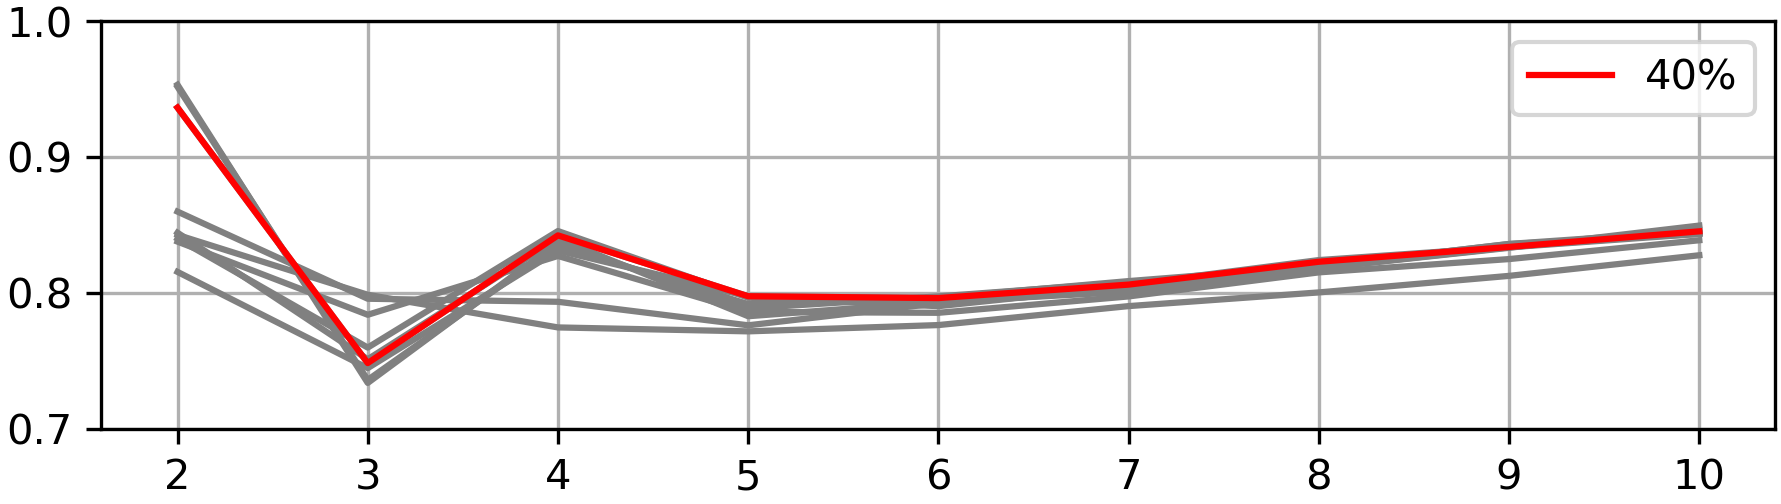
\includegraphics[width=0.8\linewidth]{pictures/Кластеры-доля}
    \\
	\caption{Доля совпадений, соотнесенная с числом кластеров}
\end{figure}


Однако сами по себе эти кривые мало что значат. Нам нужно представлять, какая из них соответствует наилучшим значениям метрики эффективности разбиения, а в силу того, что очевидного превосходства как-либо кривой из этого семейства по отношению к другим кривым этого семейства не наблюдается, делать какие-либо выводы на основании этой визуализации мы не можем.

Чтобы преодолеть это затруднение, мы вычисляем средние значения по всем числам кластеров, другими словами, усредняем строки сводной таблицы. Теперь, отталкиваясь от числовых значений, мы можем указать ту кривую, которая демонстрирует объективно более высокие усредненные показатели.

\noindent
%---------------------------------------
%---------------------------------------
\SetTblrInner{rowsep=3pt}
%---------------------------------------
\begin{longtblr}
	{
		colspec = {
			X[r,f]
			X[r,f] 
			X[r,f] 
			X[r,f] 
			X[r,f]
			X[r,f]
			X[r,f] 
			X[r,f] 
			X[r,f] 
			X[c,f]
		},
		width = \linewidth,
		rowhead = 1, 
		rowfoot = 0,
		row{odd} = {}, 
		row{even} = {},
		rows    = {font=\scriptsize},
		row{1}  = {font=\scriptsize\bfseries}
	}
	&
	10\%
	& 
	20\%
	&
	30\%
	&
	40\%
	& 
	50\%
	&
	60\%
	& 
	70\%
	&
	80\%
	&
	90\%
	\\
	\hline[1pt]
	\textbf{}   
	&0.813	&0.812	&0.809	&0.825	&0.824	&0.824	&0.814	&0.810	&0.799
	\\
	\hline[1pt]
\end{longtblr}
%---------------------------------------
\noindent
Визуально это означает, что мы усредняем каждую кривую, для чего вычисляем среднее значение кривой на всем промежутке ее изменения и заменяем кривую горизонтальной прямой (см. рис. 2).
\begin{figure}[!h]
	\centering
	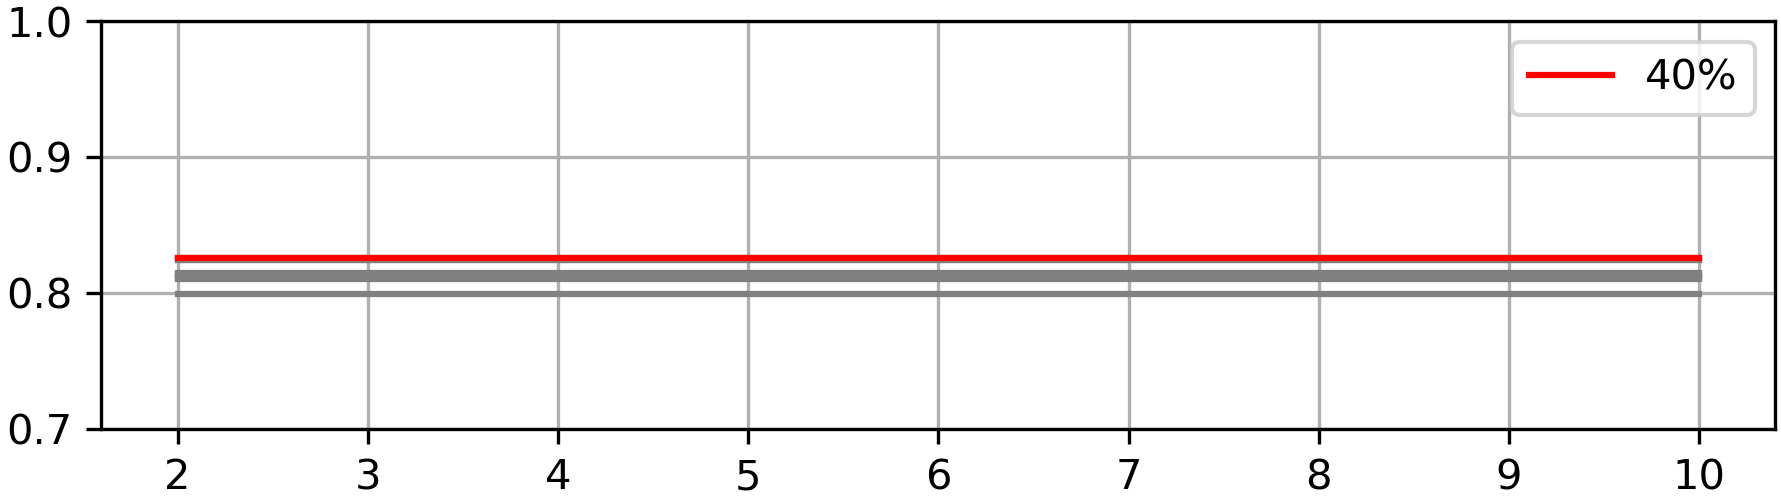
\includegraphics[width=0.8\linewidth]{pictures/Кластеры-доля. Средние}
	\\
	\caption{Доля совпадений, усредненная по всем процентам}
\end{figure}

Максимальное значение в усредненной таблице соответствует разбиению данных на тестовую и обучающую выборки в отношении 40\% к 60\% (где 40\% — объем теста). Строго говоря, отношения 40\% к 60\%, 50\% к 50\% и 60\% к 40\% дают практически неразличимые доли совпадений (см., например, рисунок 3). С практической точки зрения можно рекомендовать любое из этих соотношений. Но формально наибольшая доля совпадений возникает при объеме теста в 40\%, поэтому именно его мы выделяем как оптимальный процент разбиения данных на обучающую и тестовую выборки.



\subsection{По объему test'а}
Визуализация доли совпадений как функции от объема тестовой выборки представлена на рис. 3. Здесь девять кривых соответствуют девяти строкам сводной таблицы, и каждая кривая описывает ситуацию при фиксированном числе кластеров, на которые производится разбиение данных (от 2 до 10).
\begin{figure}[!h]
	\centering
	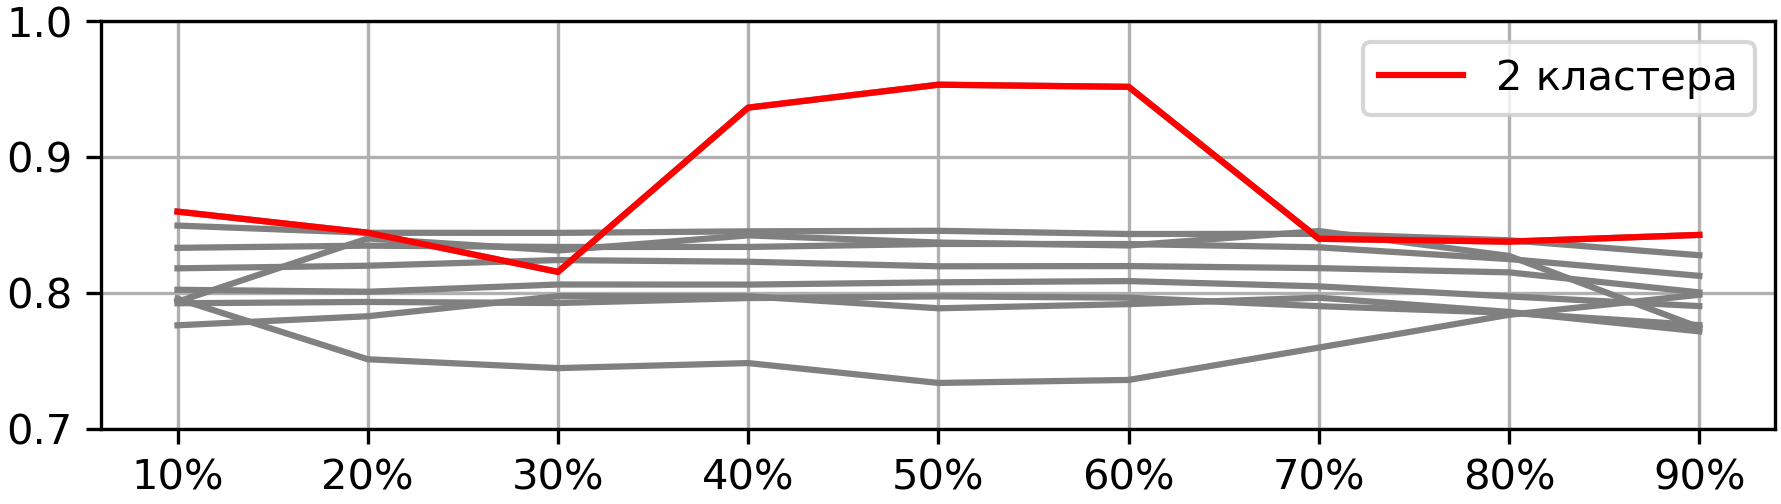
\includegraphics[width=0.8\linewidth]{pictures/Проценты-доля}
	\\
	\caption{Доля совпадений, соотнесенная с процентом test'а}
\end{figure}

Вычисляем средние доли совпадений по всем объемам тестовой выборки. Для этого усредняем столбцы сводной таблицы:

\noindent
%---------------------------------------
%---------------------------------------
\SetTblrInner{rowsep=3pt}
%---------------------------------------
\begin{longtblr}
	{
		colspec = {
			X[r,f]
			X[r,f] 
			X[r,f] 
			X[r,f] 
			X[r,f]
			X[r,f]
			X[r,f] 
			X[r,f] 
			X[r,f] 
			X[c,f]
		},
		width = \linewidth,
		rowhead = 1, 
		rowfoot = 0,
		row{odd} = {}, 
		row{even} = {},
		rows    = {font=\scriptsize},
		row{1}  = {font=\scriptsize\bfseries}
	}
	&
	2
	& 
	3
	&
	4
	&
	5
	& 
	6
	&
	7
	& 
	8
	&
    9
	&
	10
	\\
	\hline[1pt]
	\textbf{}   
	&0.875	&0.761	&0.825	&0.787	&0.791	&0.802	&0.817	&0.830	&0.842
	\\
	\hline[1pt]
\end{longtblr}
%---------------------------------------
\noindent

Визуально это означает, что каждая кривая становится горизонтальной прямой (см. рис. 4).



\begin{figure}[!h]
	\centering
	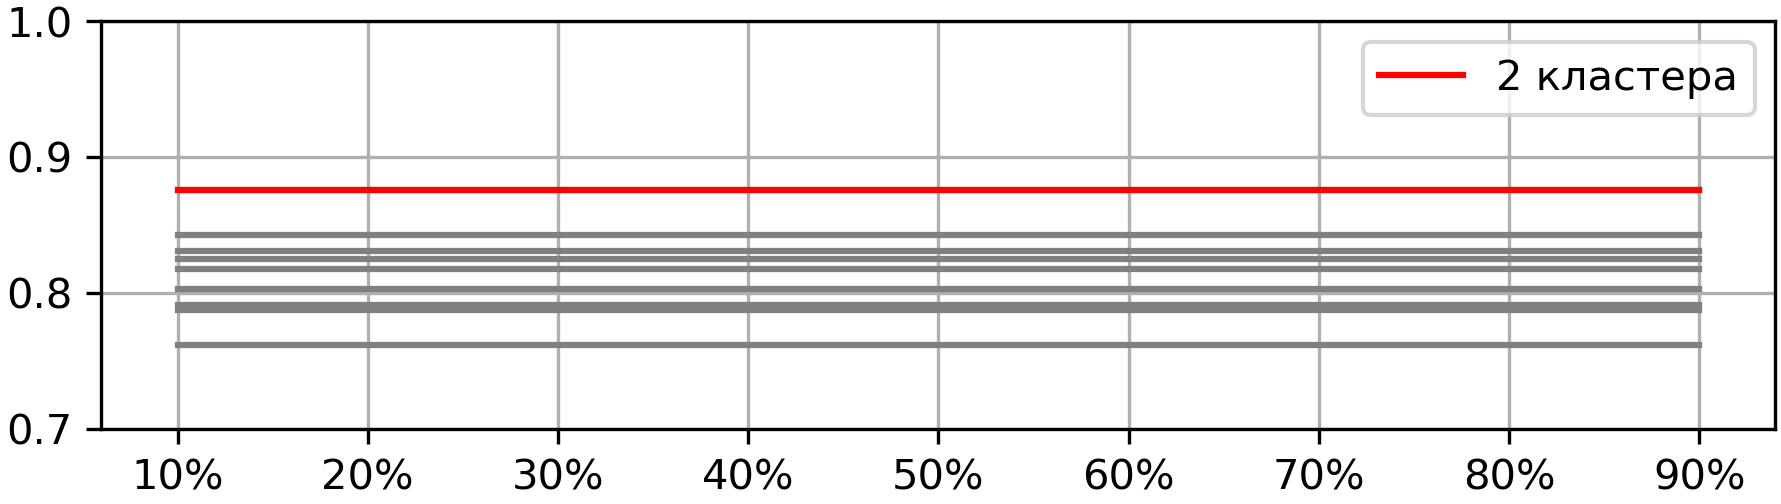
\includegraphics[width=0.8\linewidth]{pictures/Проценты-доля.Средние}
	\\
	\caption{Доля совпадений, усредненная по числам кластеров}
\end{figure}


Наиболее высокая прямая (или, что то же самое, максимальное значение в усредненной таблице) соответствует двум кластерам.


\section{Выводы}
	
Кластеризация данных используется в широком спектре задач и отраслей, включая маркетинг, медицину, обнаружение мошенничества и многие другие (см. [5]). Определение правильного числа кластеров помогает принимать правильные решения на основе кластерных анализов, такие как создание сегментов покупателей, выявление характерных поведенческих паттернов или предсказание рисков и мошеннических действий.

Число кластеров напрямую влияет на качество и интерпретируемость кластеризации. Неправильное определение числа кластеров может привести к объединению сильно различающихся групп в один кластер или к разделению однородной группы на несколько кластеров. Правильно определенное число кластеров помогает обнаружить скрытые шаблоны, взаимосвязи и сходства в данных (см. [2], [5], [6]).

Определение числа кластеров является серьезной задачей, один из подходов к решению которой был продемонстрирован в этой статье. Применение нашего метода к реальным данным о потреблении контента потребителями одного из ведущих хостингов показало его работоспособность в условиях, когда какие-либо доводы со стороны экспертов предметной области отсутствуют, и решение о разбиении принимается формально, на основании числовых данных, но не их интерпретации.


\section{Литература}

\begin{enumerate}
	\item Хейдт М. Изучаем Pandas / М. Хейдт;  — Москва: ДМК Пресс, 2018. — 438 с.
	\item Бурков А. Машинное обучение без лишних слов / А. Бурков;  — СПб: Питер, 2020. — 192 с.
	\item Вьюгин, В. В. Математические основы теории машинного обучения и прогнозирования / В. В. Вьюгин; — М.: МЦИМО. — 2013. — 387~с.
	\item Бринк Х. Машинное обучение / Х. Бринк, Дж. Ричардс, М. Феверолф  — СПб.: Питер, 2017. — 336 с.
	\item Байков И.И., Семерова Е.А., Курмуков А.И. Метод ансамблирования алгоритмов кластеризации для решения задачи совместной кластеризации // Сенсорные системы. 2021. Т. 35. № 1. С. 43--49.
	\item Паксашвили С.А. Тестирование алгоритма кластеризации k-means в решении задачи кластеризации финансовых операций // В сборнике: СНК-2022. Материалы LXXII открытой международной студенческой научной конференции Московского Политеха. Москва, 2022. С. 347--353.
	
\end{enumerate}



\end{document}